\acrfull{io}, as the name suggests, are the inputs and outputs of a control system. Inputs are often referred to as sensors as they are devices that translate a real world signal into something that the \acrshort{cpu} can make sense of - this typically consists of some sort of electrical signal (Voltage or Current). Outputs, on the other hand, are often referred to as "final control elements" or "actuators". Output devices are how the control system is able to interact with the outside world.\\
There are four main types of \acrshort{io}:


\begin{description}
    \item\textbf{Digital Inputs} - Binary input signals (On or Off).
    \item\textbf{Digital Outputs} - Binary output signals (On of Off).
    \item\textbf{Analog Inputs} - Variable electrical (voltage or current) inputs signals.
    \item\textbf{Analog Outputs} - Variable electrical (voltage or current) output signals.
\end{description}
    
    
The lolly machine \acrshort{io} is comprised of digital inputs and outputs. This section will provide a brief overview to all different types of digital \acrshort{io} that can be found on the lolly machine


\subsection{Inputs}
    \subsubsection{Limit Switches}
        Magnetically activated limit switches manufactured by \acrshort{smc} provide actuator position feedback. There are two limit switches installed on each actuator, one that activates when the actuator is fully extended and the other when it is fully retracted. The limit switches are installed within a track on the actuator and held in place by a small grub screw - this can be seen in Figure \ref{fig:rejectAct}.
        The limit switches have an internal solid state circuit that is activated when the piston is adjacent. The piston is made from a magnetic ferrous material which is what allows the switch to activate. 
        Figure \ref{fig:autSwShm} shows the internal electrical schematic of the \acrshort{smc} limit switches.
        
        \begin{figure}[H]
            \centering
            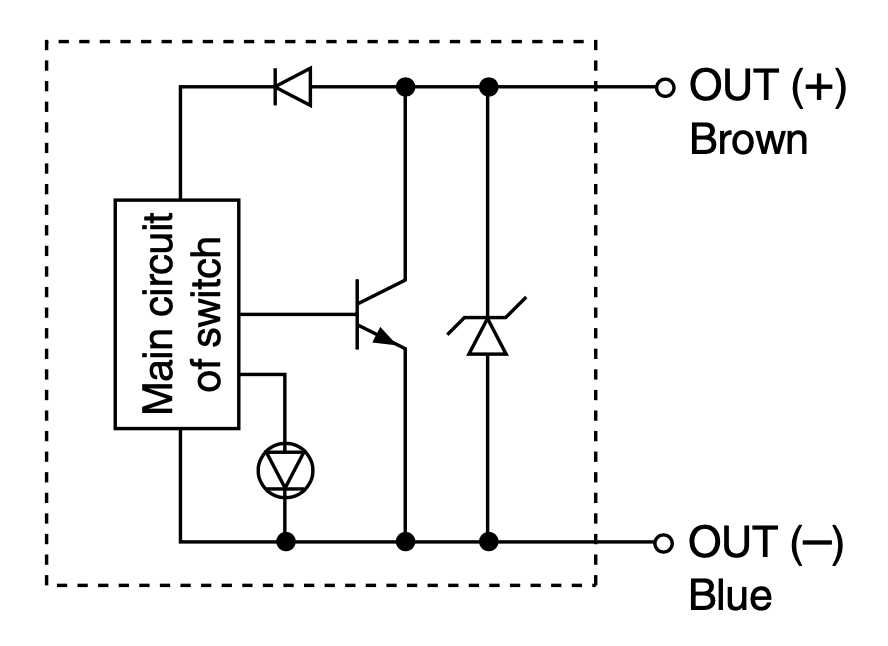
\includegraphics[scale = 0.4]{2_images/autSwShm.png}
            \caption{Internal electrical schematic of an \acrshort{smc} limit switch~\cite{smcRot}.}
            \label{fig:autSwShm}
        \end{figure}
    
        
        %PHOTO
    
    \subsubsection{Proximity Sensors}
        Two proximity sensors are installed on the lolly machine. The sensors determine whether or not a lolly is in situ. The proximity sensors installed on the lolly machine are capacitive; this allows the sensors to detect ferrous and non-ferrous materials. Figure \ref{fig:proxSens} illustrates the general function of a proximity sensors. In the case of the lolly machine, the proximity sensors are \acrshort{nc} which means that the output is on when the target is detected and off while the target is not.
    \begin{figure}[H]
    \begin{minipage}{0.35\textwidth}
        \centering
            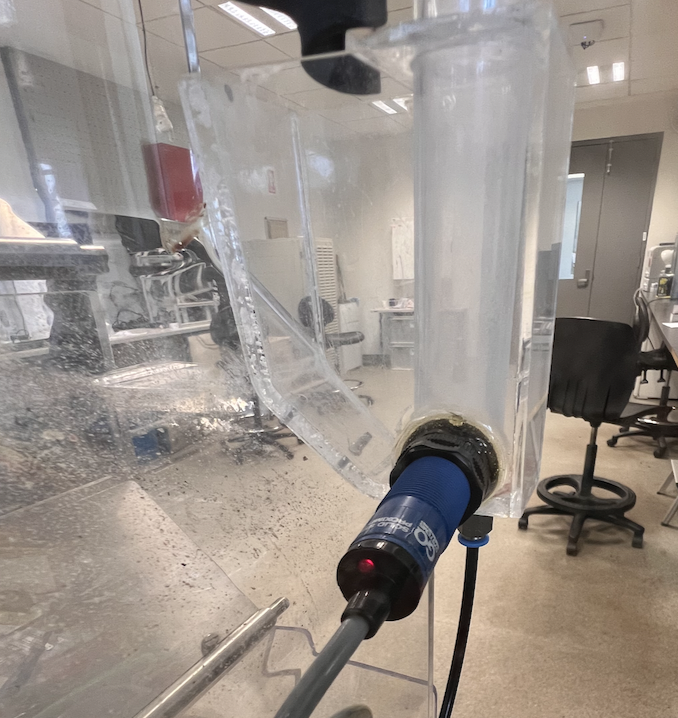
\includegraphics[scale = 0.4]{2_images/rejectProx.png}
            \caption{Lolly machine proximity sensor used to detect when a lolly is in the reject bucket.}
            \label{fig:rejectProx}
    \end{minipage}\hfill
    \begin{minipage}{0.35\textwidth}
        \centering
        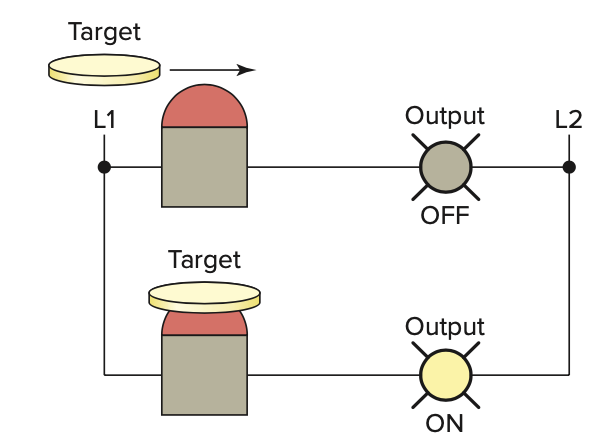
\includegraphics[width = 0.9\textwidth]{2_images/proxSens.png}
        \caption{Typical function of a proximity sensor \cite{petruzella2017programmable}.}
        \label{fig:proxSens}
    \end{minipage}\hfill 
    \end{figure}
 \newpage
    
    \subsubsection{Colour Sensors}
        Colour sensors determine colour through the hue, chrominance and luminance of an object \cite{sickCs}.
        Although the colour sensors used on the lolly machine can’t actually detect the complete range of colours which can be seen by us, the two colours sensors (3 digital signals from one sensor, and 1 digital signal from the second), are able to be “trained/calibrated” to provide an indication of a number of different colour matches.
        Figure \ref{fig:cs1} shows the electrical connections of one of the colour sensors while Figure \ref{fig:colSens} shows a picture of the colour sensors installed on the machine.

        \begin{figure}[H]
            \centering
            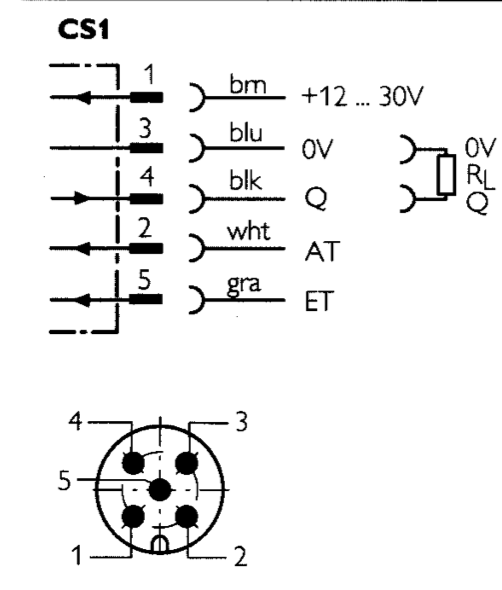
\includegraphics[scale = 0.4]{2_images/cs1.png}
            \caption{Electrical connections for a single output colour sensor \cite{sickCs}.}
            \label{fig:cs1}
        \end{figure}     
        
        \begin{figure}[H]
            \centering
            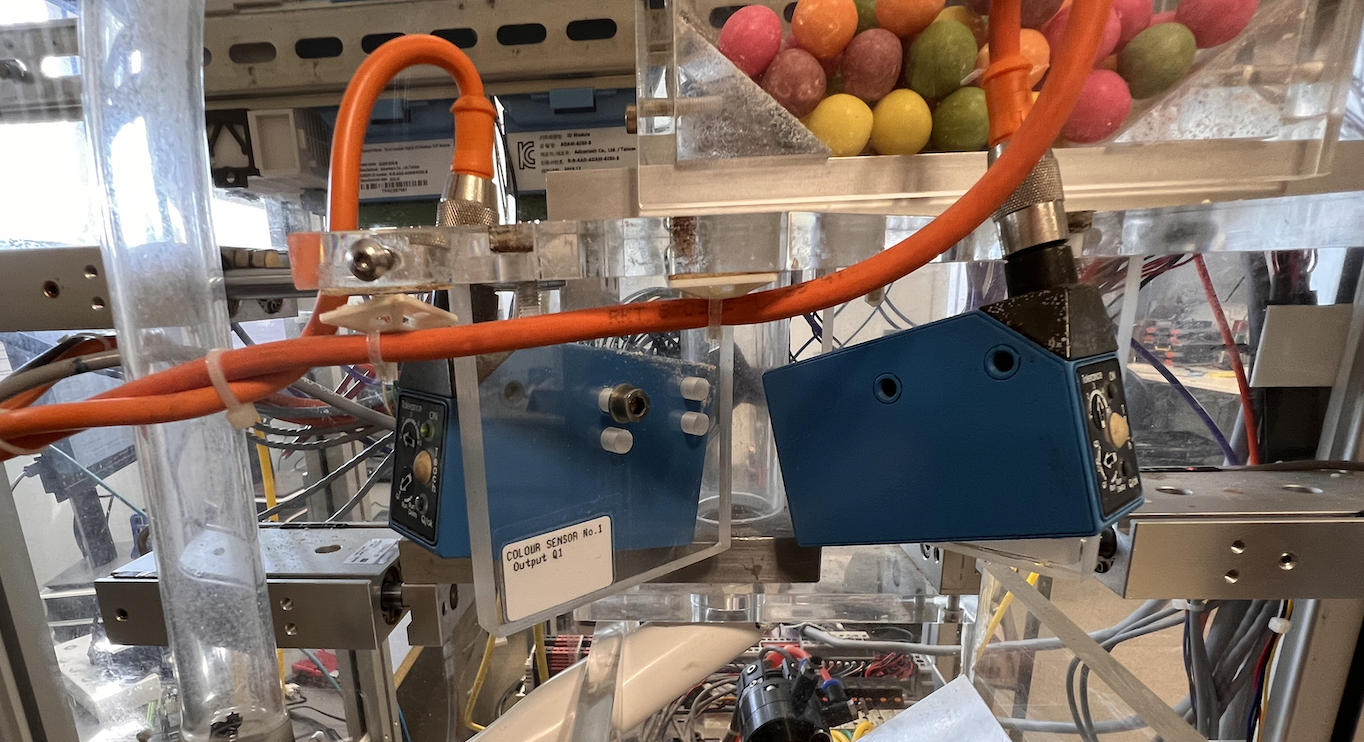
\includegraphics[scale = 0.4]{2_images/colSens.png}
            \caption{The two lolly machine colour sensors.}
            \label{fig:colSens}
        \end{figure}       

    
    \subsubsection{Buttons}
    Physical push buttons provide an interface between the operator and the machine where different buttons are linked to different machine functions. For example, an \acrfull{estop}, when pressed, will halt the operation of the machine and put it into error mode. While in error mode, the machine will cease to operate until it has been an given instruction by the user that it is safe to do so. The \acrshort{estop} is a \acrshort{nc} contact while the rest of the buttons on the machine are \acrshort{no}.
\newpage
    %Find a figure of a NO button - can probably find in the PLC book
    
\subsection{Outputs}
    \subsubsection{Solenoids - Pneumatic Valve}
    All pneumatic actuators on the lolly machine are activated by pneumatic control valves. The control valves are activated by an internal solenoid driven pilot valve.  The output device, from the perspective of the \acrshort{plc}, is the solenoid. The fundamental components of a solenoid are a wire coil and ferrous core. The ferrous core is located within the coil. When a \acrshort{dc} voltage is applied to the coil it behaves like a magnet, this is called an electromagnet. When the solenoid is switched, the ferrous core moves from one end of the solenoid housing to the other. The core is connected to the pilot valve which provides the necessary mechanical action to change the valve position, which in turn, moves the actuator. 
    
        \begin{figure}[H]
            \centering
            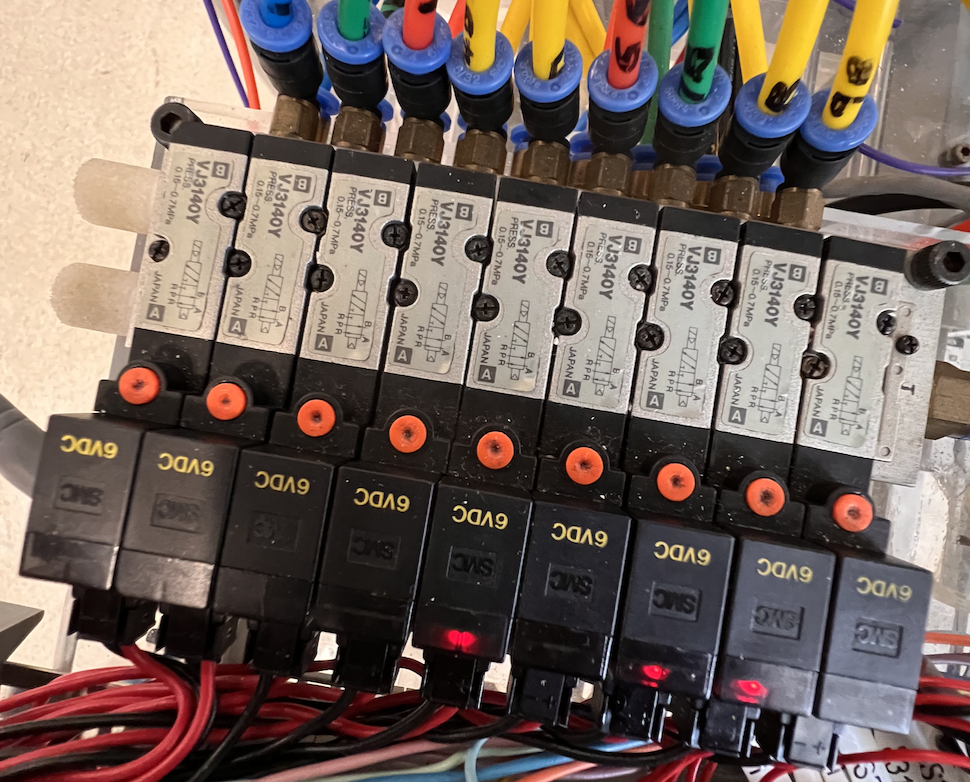
\includegraphics[scale = 0.5]{2_images/controlValvesPic.png}
            \caption{Solenoid pneumatic control valves mounted on manifold.}
            \label{fig:controlValvesPic}
        \end{figure} 
    \newpage
    \subsubsection{\acrshort{led} Indicators}
        A number of \acrshort{led} based lights are used on the lolly machine. The \acrshort{led}s are linked to specific machine states and will either be on, off  or flashing. \acrshort{led}s are robust, lasting much longer than previously used incandescent lights. As most \acrshort{led}s require only a couple of volts, all have internal series resistors which allows all \acrshort{led}s on the lolly machine to be directly controlled and switched by the \acrshort{plc}.
        
        
        \begin{figure}[H]
            \centering
            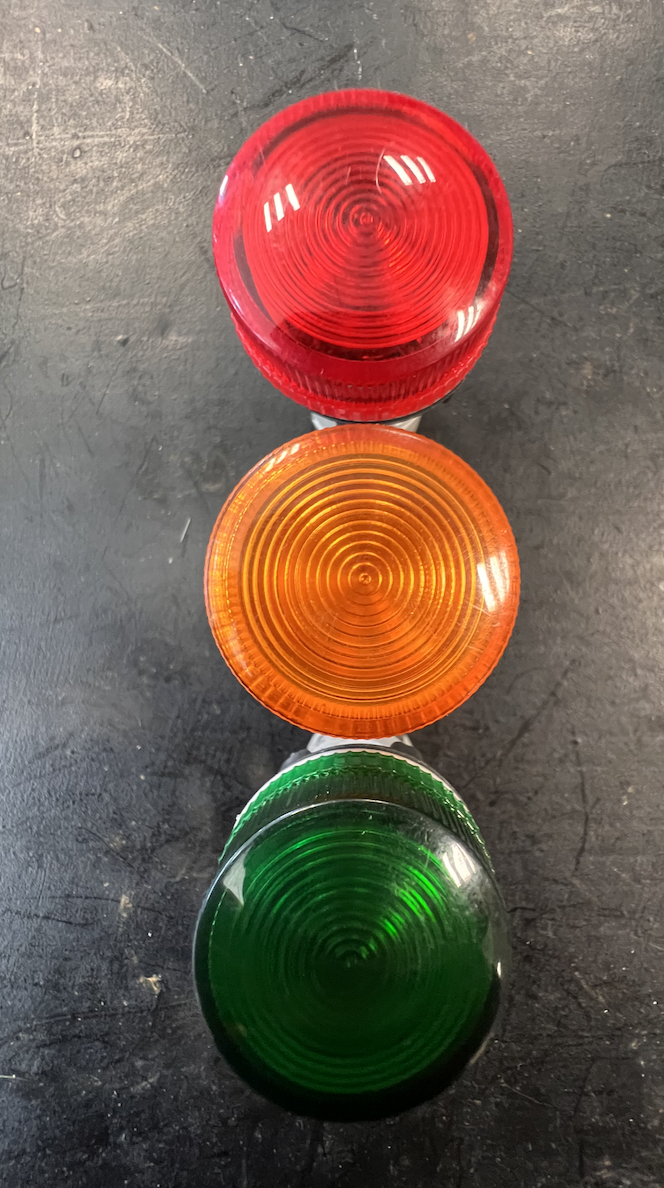
\includegraphics[scale = 0.3]{2_images/leds.png}
            \caption{Lolly machine \acrshort{led}s}
            \label{fig:leds}
        \end{figure} 
        
